\section{Overview}

\begin{frame}[c]{Learning Goals} 
    \large
    \begin{itemize}[<+(1)->]
        % \item Gain familiarity with the transformer architecture and understand how it works
        \item Gain familiarity with tokens and embeddings in the context of
            transformer architectures
        \item Understand how Attention works
        \item Awareness of common extensions and usages
        \item Recognize its limitations
    \end{itemize}
    \pause
    \textbf{Key Takeaway:} Transformers are a powerful and flexible
    architecture, suitable for most sequence-to-sequence tasks.
    \pnote{
        sequence to sequence also includes everything \\
        where an intermediate sequence is an embedding
    }
\end{frame}

\addtocounter{framenumber}{1}
\begin{frame}[standout]
    \huge
    Ask if you have questions \\
    or anything is unclear
    \pnote{
        I will be jumping around different topics a bunch \\
        Ask immediately if anything is unclear
    }
\end{frame}

\begin{frame}[c]{Overview}
    \begin{figure}
        \begin{columns}
            \column{0.8\linewidth}
            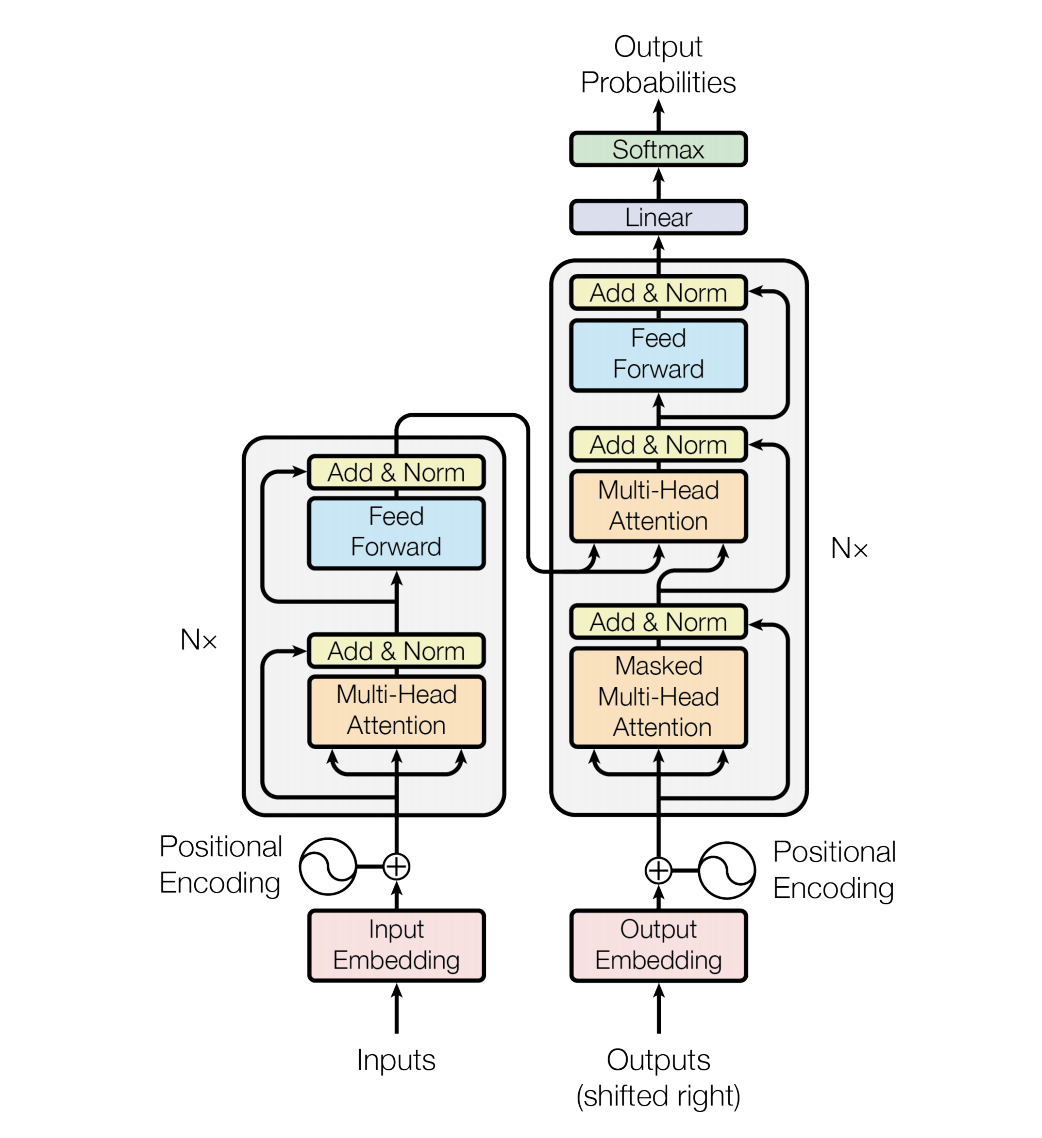
\includegraphics[height=0.9\textheight]{transformer}
            % \column{0.2\linewidth}
            \column{\dimexpr0.15\linewidth+9em}
            \raisebox{3em}{\gray{Image Source: \cite{vaswani_attention_2017}}}
        \end{columns}
    \end{figure}
\end{frame}
